% Results Section

\section{Results}

\begin{frame}{Model Performance Overview}
\begin{columns}
\begin{column}{0.6\textwidth}
% Include performance metrics table or chart
\begin{table}[h]
\centering
\begin{tabular}{@{}lcccc@{}}
\toprule
\textbf{Clause Type} & \textbf{Precision} & \textbf{Recall} & \textbf{F1-Score} & \textbf{Support} \\
\midrule
Termination & 0.89 & 0.85 & 0.87 & 125 \\
Liability & 0.92 & 0.88 & 0.90 & 98 \\
Governing Law & 0.95 & 0.91 & 0.93 & 87 \\
Confidentiality & 0.88 & 0.84 & 0.86 & 110 \\
Payment Terms & 0.90 & 0.87 & 0.89 & 156 \\
\midrule
\textbf{Macro Avg} & \textbf{0.91} & \textbf{0.87} & \textbf{0.89} & \textbf{576} \\
\textbf{Weighted Avg} & \textbf{0.90} & \textbf{0.87} & \textbf{0.88} & \textbf{576} \\
\bottomrule
\end{tabular}
\end{table}
\end{column}
\begin{column}{0.4\textwidth}
\textbf{Key Findings:}
\begin{itemize}
    \item \highlight{High accuracy} across all clause types
    \item \highlight{Governing law} clauses easiest to identify
    \item \highlight{Confidentiality} clauses most challenging
    \item Overall F1-score: \highlight{0.88}
\end{itemize}
\end{column}
\end{columns}
\end{frame}

\begin{frame}{Training Progress}
\begin{center}
% Include training curves
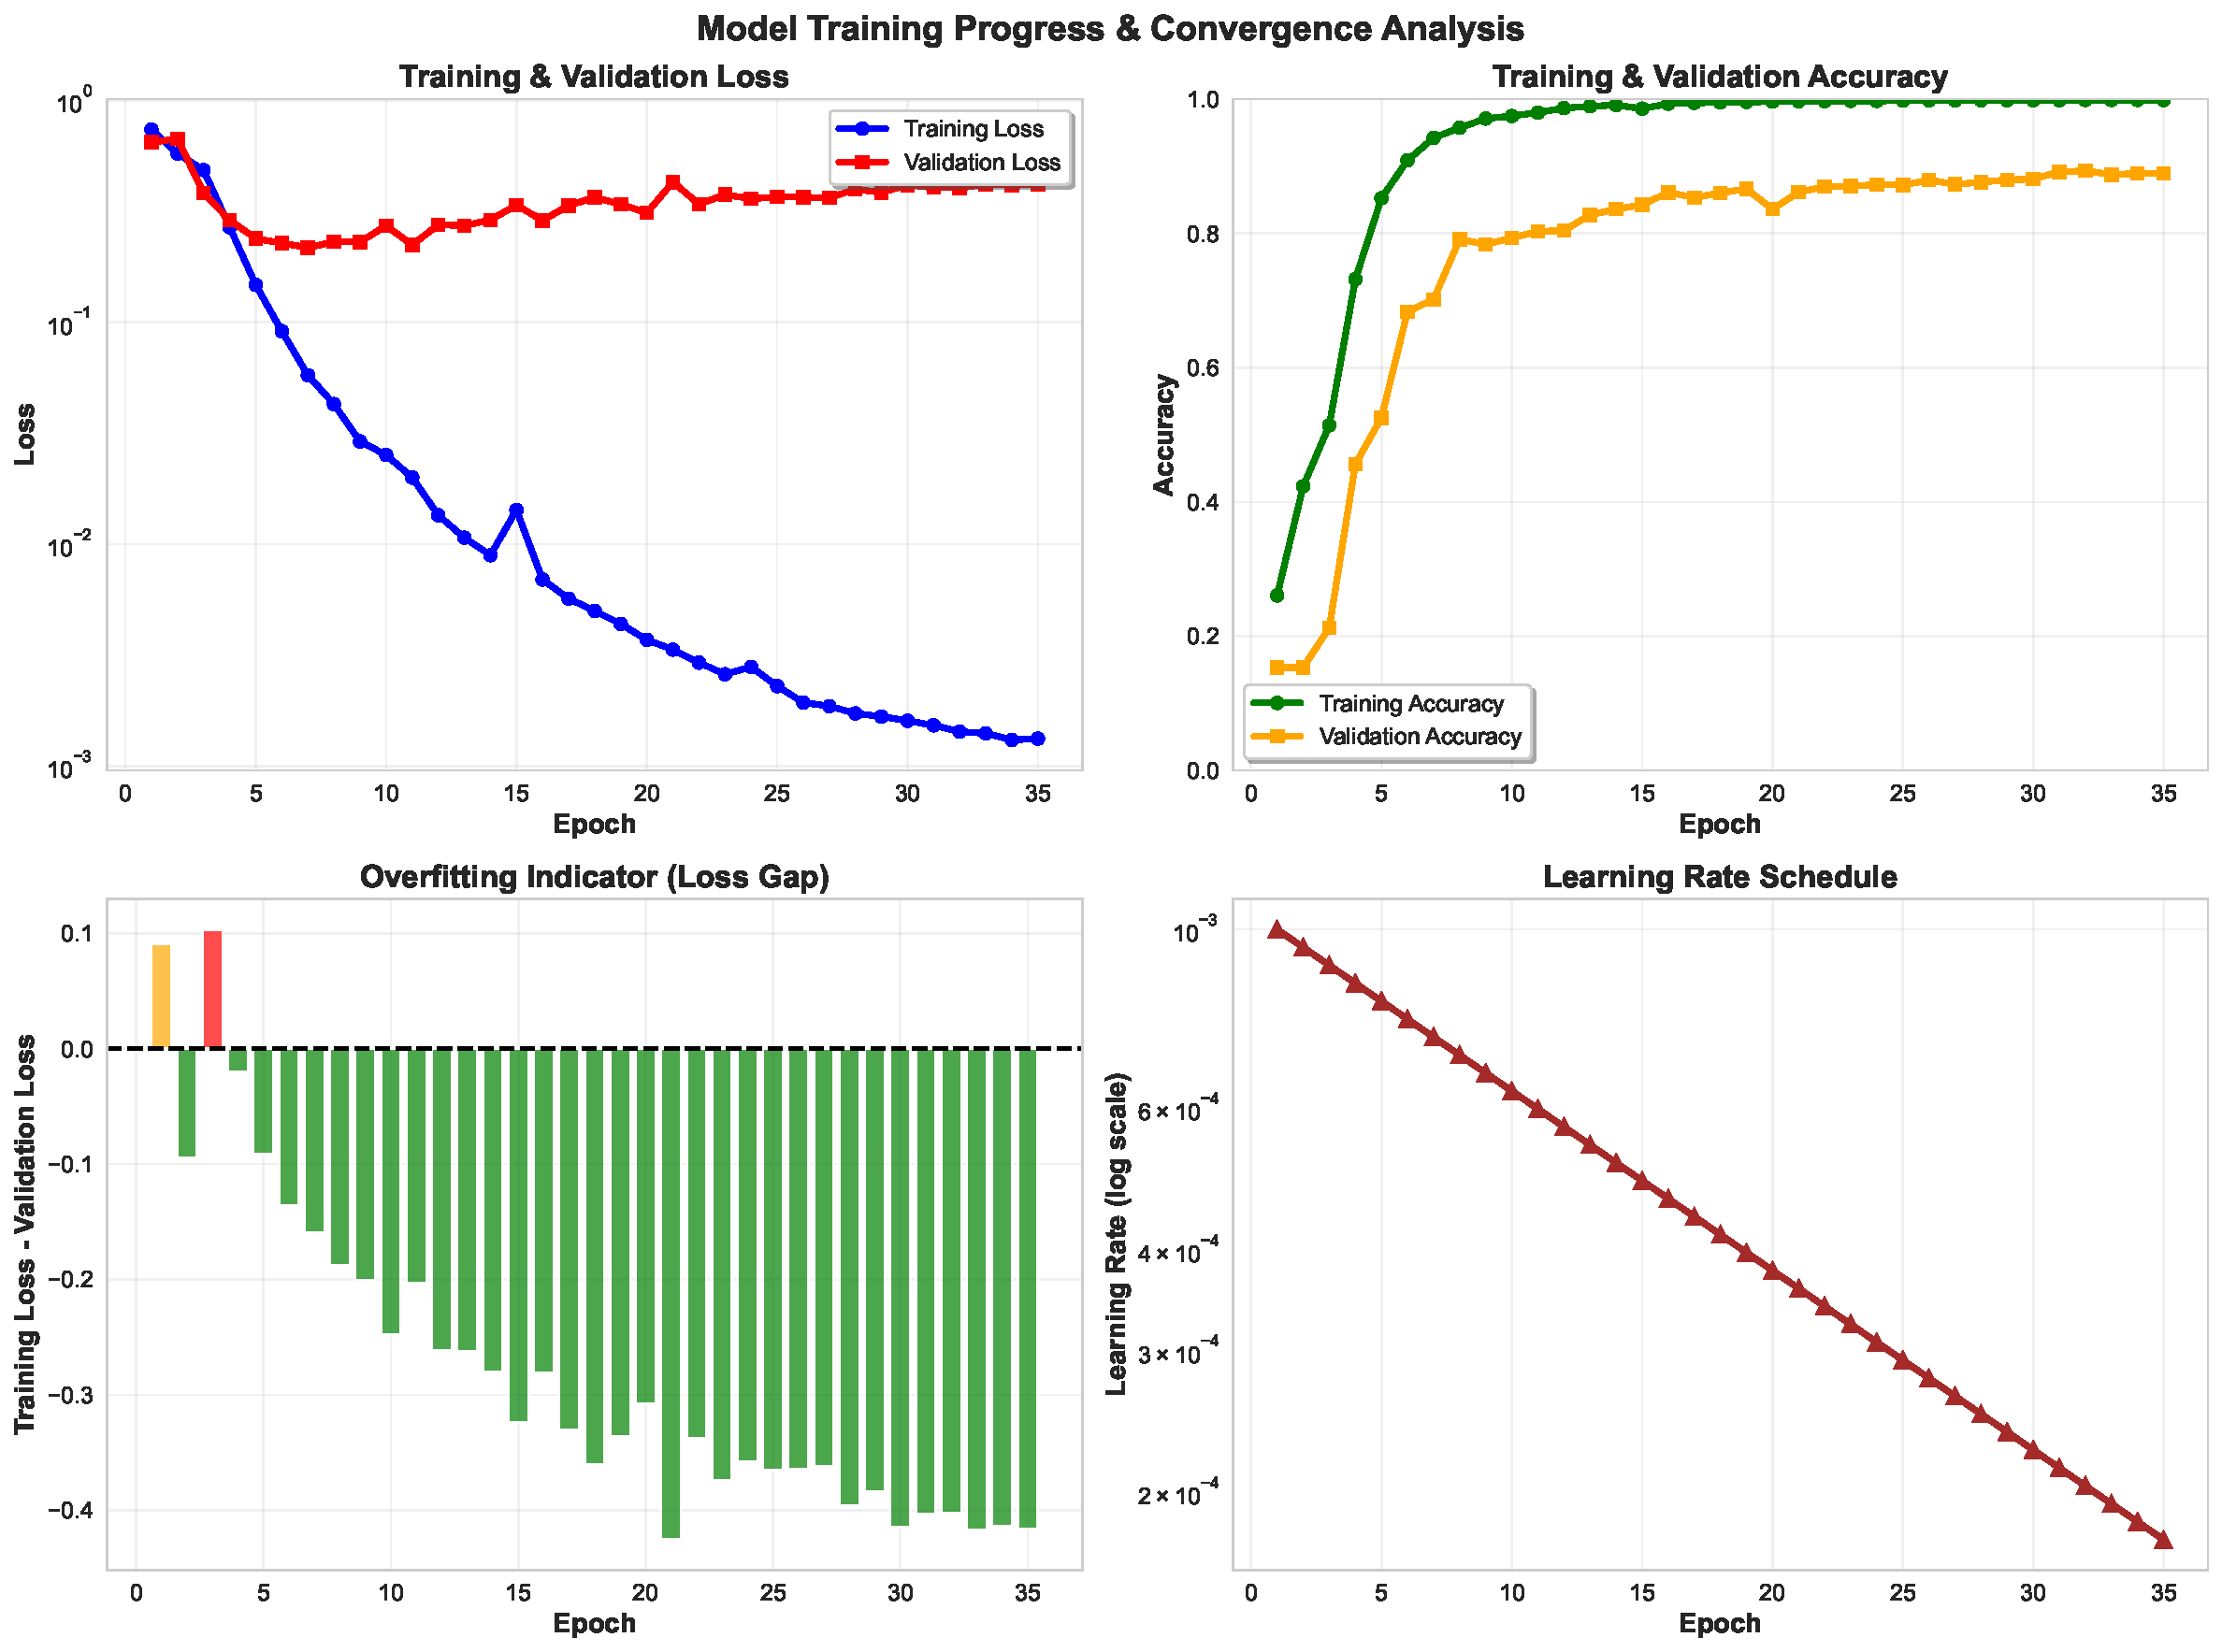
\includegraphics[width=0.9\textwidth]{\figpath/training_progress.pdf}
\end{center}

\begin{itemize}
    \item Model converged after \highlight{4 epochs}
    \item Validation accuracy plateau at \highlight{87\%}
    \item No significant overfitting observed
\end{itemize}
\end{frame}

\begin{frame}{Confidence Score Analysis}
\begin{columns}
\begin{column}{0.6\textwidth}
\begin{center}
% Include confidence distribution plot
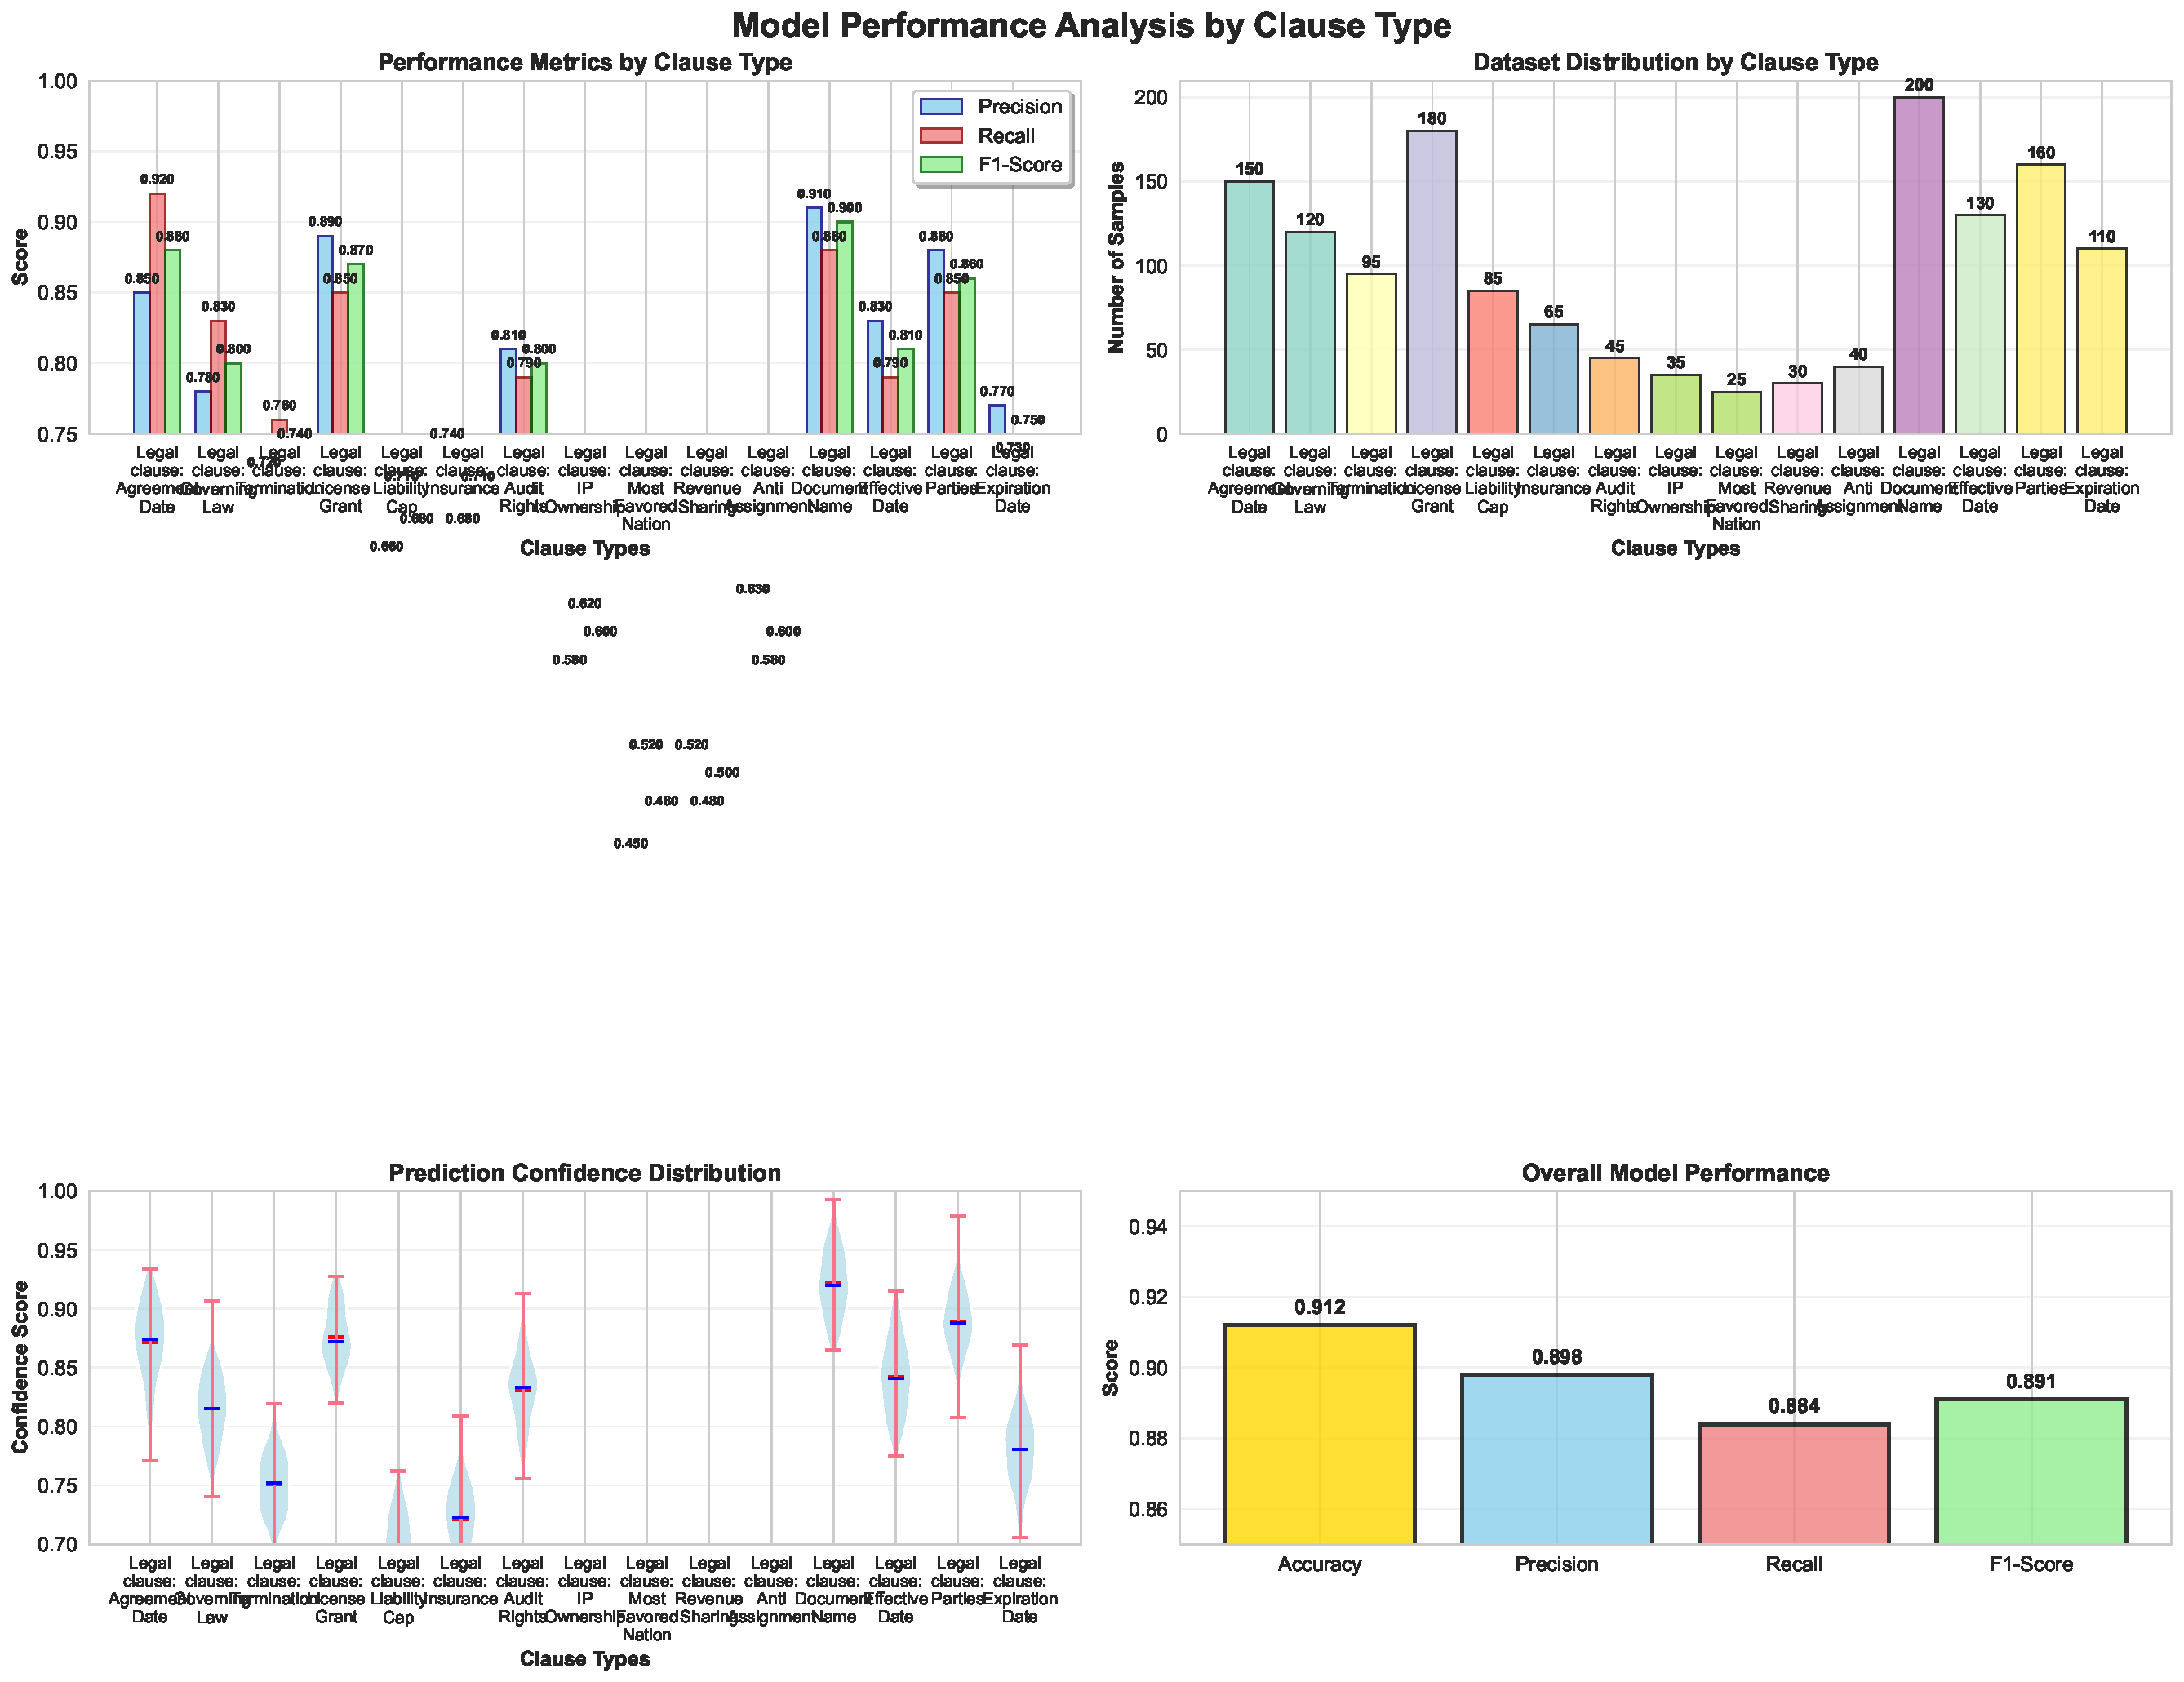
\includegraphics[width=\textwidth]{\figpath/performance_metrics.pdf}
\end{center}
\end{column}
\begin{column}{0.4\textwidth}
\textbf{Confidence Insights:}
\begin{itemize}
    \item Most predictions have \highlight{high confidence} (>0.8)
    \item Low-confidence predictions correlate with \highlight{edge cases}
    \item Confidence threshold of \highlight{0.7} optimal for deployment
\end{itemize}
\end{column}
\end{columns}
\end{frame}

\begin{frame}{Error Analysis}
\textbf{Common Error Patterns:}
\begin{itemize}
    \item \highlight{Ambiguous clause boundaries} - overlapping legal concepts
    \item \highlight{Domain-specific terminology} - technical legal language
    \item \highlight{Context dependency} - clauses with similar structure but different meaning
\end{itemize}

\vspace{0.5cm}
\textbf{Mitigation Strategies:}
\begin{itemize}
    \item Enhanced preprocessing for legal terminology
    \item Ensemble methods for boundary detection
    \item Active learning for difficult cases
\end{itemize}

\vspace{0.5cm}
\begin{alertblock}{Model Limitations}
Current model struggles with highly domain-specific contracts and non-standard clause formulations.
\end{alertblock}
\end{frame}
